\documentclass[a4paper,12pt]{article}
\usepackage{graphicx}
\usepackage{float}
\usepackage[a4paper, margin=1in]{geometry}

\begin{document}

\title{Is Florida Getting Warmer? - An Analysis}
\author{Yijie Jiao}
\date{\today}
\maketitle

\begin{abstract}
This document presents the results of a permutation analysis conducted to explore the correlation between years and temperature in Florida, aiming to address the question: "Is Florida getting warmer?"
\end{abstract}

\section*{Results}
The observed Pearson correlation coefficient between the years and temperature in Florida is \textbf{0.372}. To test the significance of this correlation, a permutation analysis with 10,000 iterations was conducted, reshuffling the temperature data to generate a distribution of random correlation coefficients.

\begin{figure}[H]
    \centering
    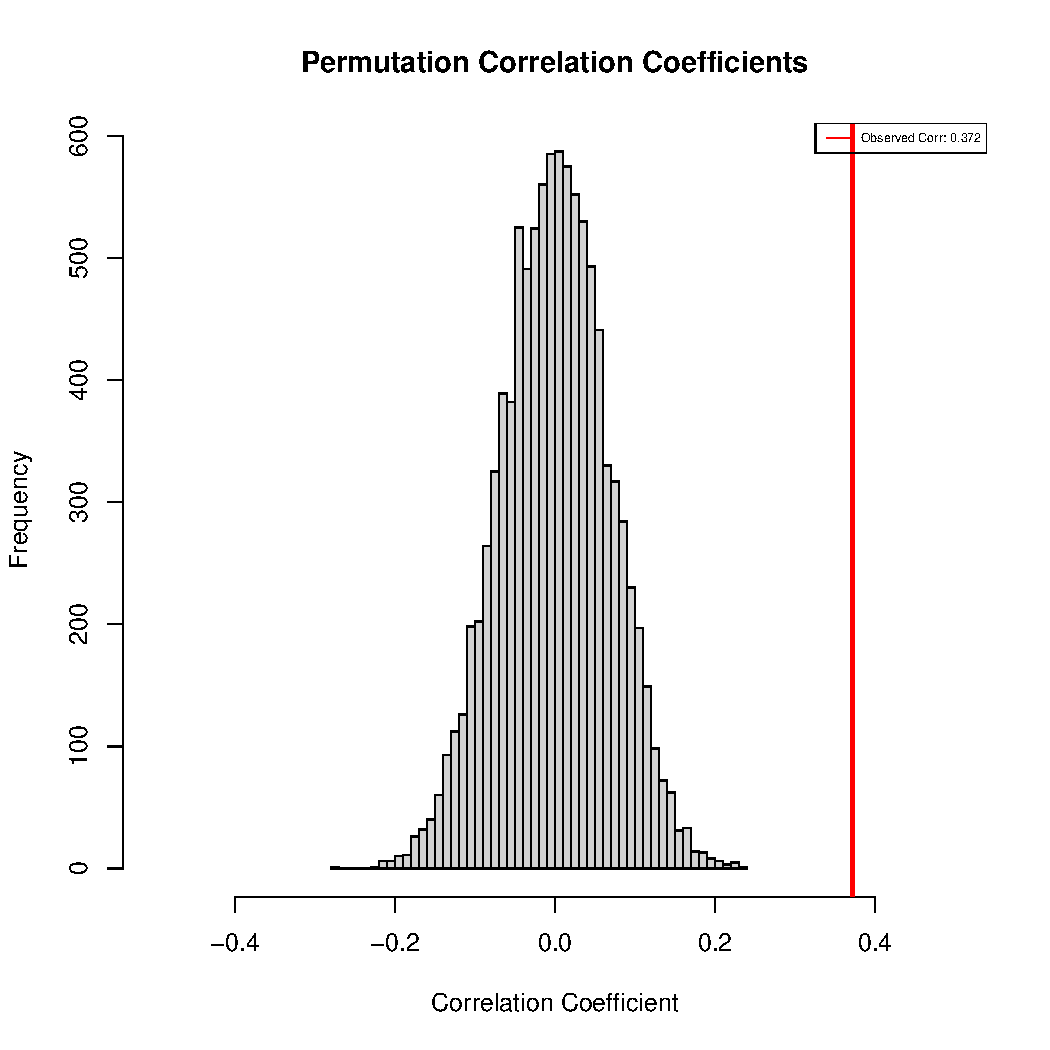
\includegraphics[width=\textwidth]{correlation_histogram.pdf} % Replace with actual file path
    \caption{Histogram of permutation correlation coefficients with the observed value indicated by the red line.}
\end{figure}

The approximate p-value obtained from this analysis is \textbf{0}, suggesting that the correlation observed is SIGNIFICANT.

\section*{Interpretation}
The analysis suggests that there is a POSITIVE correlation between the years and temperature in Florida, implying that Florida is IS getting warmer over time.

\end{document}
